\chapterauthor{Ricardo Krause}
\chapter{Projektstart}

Dieses Kapitel wurde von Herrn Krause erstellt und betreut. Es beschreibt die Startphase des Projektes und zählt auf, welche Tätigkeiten und Entscheidungen vor Beginn des eigentlichen Projektes durchgeführt wurden. Es werden die Punkte Projektauftrag, Projektplan, Versionsverwaltung, Projektkommunikation und Dokumentenmanagement beschrieben.

\section{Projektauftrag}

Das grundlegende Dokument für jedes Projekt ist der Projektauftrag, dieser Auftrag beinhaltet alle relevanten Parameter und Eckdaten des Projektes.

\begin{description}
\item[Projekttitel:] Der Arbeitstitel des Projektes.
\item[Projektnummer:] Eine in der Regel einzigartige Nummer zur Identifikation eines Projektes.
\item[Projektart:] Unterscheidung von verschiedenen möglichen Projekttypen.
\item[Projektleiter:] Bindeglied zwischen Kunden und Entwicklern mit überwachender und steuernder Tätigkeit.
\item[Projektauftraggeber:] Der Auftraggeber des Projektes.
\item[Projektkunden:] Können vom Auftraggeber abweichen und auch mehrere sein.
\item[Projektdauer:] Legt den zeitlichen Rahmen des Projektes fest.
\item[Ausgangssituation/Problembeschreibung:] Das beschreibt den aktuellen Zustand und das Problem, welches mit dem Projekt gelöst werden soll.
\item[Projektgesamtziel:] Zusammengefasste Beschreibung des Projektes mit dem zu erreichenden Ziel.
\item[Projektteilziele und -ergebnisse:] Detaillierte Auflistung der einzelnen Teilziele, mit den messbaren zu erreichenden Ergebnissen.
\item[Nicht-Ziele / Nicht-Inhalte:] Abgrenzung des Projektes.
\item[Meilensteine:] Ereignisse des Projektes, welche zu unterschiedlichen Daten erreicht werden müssen, um das Projekt erfolgreich abzuschließen.
\item[Randbedingungen und Projekt Kontext:] Nebenbedingungen, welche meist nicht direkt vom Projektteam beeinflussbar, aber notwendig zum Erreichen des Projektzieles sind.
\item[Projektklassifizierung:] Parameter, welche das Projekt als Ziffer beschreiben und somit eine Vergleichbarkeit zwischen anderen Projekten schaffen.
\item[Projektorganisation:] Beinhaltet das Projektteam, weitere beteiligte Personen.
\item[Projektressourcen:] Alle für das Projekt zur Verfügung stehenden Ressourcen, beinhalten Personal und Material.
\item[Projektbudget:] Das zur Verfügung stehende Budget.
\item[Wirtschaftlicher oder sonstiger Nutzen:] Dieser Parameter ist meist wichtig für die Entscheider eines Projektes und soll den Gewinn durch das Projekt aufzeigen.
\item[Projektrisiken und -unsicherheiten:] Zeigt alle Risiken auf, welche zu einen Scheitern des Projekt führen könnten.
\item[Projektentscheidung:] Das Projekt muss vor Beginn von einer Entscheidungsbefugten Person freigeben werden.
\item[Sonstige relevante Informationen:] Weitere wichtige Information.
\item[Anlagen:] Weitere Dokumente, welche das Projekt betreffen.
\end{description}

Der Projektantrag wurde von Herr Krause aufgesetzt, die Inhalte wurden gemeinsam erarbeitet und mit den Projektbeteiligten Personen abgestimmt. Der ausgearbeitete Antrag befindet sich im Anhang

\section{Projektplan}
Nach dem der Projektantrag erstellt wurde und die Ziele des Projektes bekannt waren, wurde ein detaillierter Projektplan kreiert. Dieser Plan wurde mit dem Open Source Tool \textit{OpenProj}\footnote{Link zum Projekt  \url{http://www.serena.com/index.php/en/products/pod-update/}} erstellt und befindet sich ebenfalls im Anhang.\\
Der Projektplan beinhaltet alle erforderlichen Tätigkeiten und ermöglichte eine Abschätzung ob das Projekt mit den gegebenen Ressourcen in der Zeit durchführbar ist.

\section{Versionsverwaltung}
Als weiterer fundamentaler Pfeiler dieses Projektes wurde ein Versionsverwaltungssystem eingerichtet, welches dem Team ermöglichte, ohne größere Probleme gemeinsam an dem Projekt zu arbeiten, ohne Gefahr zu laufen, die erstellten Artefakte\footnote{Arbeitsergebnis in einem Projekt} zu beschädigen.\\
Die Wahl fiel auf das Open Source Tool \textit{GIT}\footnote{Link zum Projekt \url{https://git-scm.com/}}, welches als verteiltes Versionsverwaltungssystem für die Software Komponenten und Dokumentation eingesetzt wird.\\
Das System GIT wurde gewählt, da es schon mehreren Mitgliedern des Entwicklungsteams bekannt war und eine Vertiefung mit dem Umgang dieses Tools gewünscht wurde.\\
Durch den zusätzlichen Einsatz von \textit{Github} \footnote{Link zum Projekt \url{https://github.com/}}, welches ein Web-Interface für das eingesetzte GIT bietet, wurde es ebenfalls ermöglicht untereinander die Software Artefakte zu testen und direkt über Issues\footnote{engl. für Problem oder Angelegenheit}, Probleme und Änderungswünsche zu berichten.\\
Die grobe Erstellung des Projektes auf Github übernahm der Herr Krause, die interne Struktur der einzelnen Arbeitspakete wurde von dem Herr Kölbl erledigt. 


\section{Kommunikation}
Für die Kommunikation der Projektgruppe wurde das Open Source Tool \textit{Slack}\footnote{Link zum Projekt \url{https://slack.com/}} eingesetzt. Dieses Werkzeug ermöglichte es gemeinsam und Themenorientiert zu kommunizieren und erleichterte durch Schnittstellen zur Versions- und Dokumentenverwaltung die erforderlichen Workflows.\\
Es wurde für jedes Arbeitspaket ein eigener Kommunikationsbereich eingerichtet und Mitglieder, welche in einen bestimmten Bereich involviert oder interessiert waren, konnten diesen Bereichen beitreten und miteinander diskutieren.\\
Das Kommunikationswerkzeug wurde vom Herrn Krause eingerichtet.

\section{Dokumentenmanagement}
Im Team wurde entschieden, dass der Großteil der Dokumente für das Projekt nicht in die Versionsverwaltung gehört, weshalb für die Verwaltung dieser Dokumente der Online Speicherdienst \textit{Dropbox}\footnote{Link zum Anbieter \url{https://www.dropbox.com/home}} gewählt wurde. Dieses System wird bereits von den beteiligten Studenten eingesetzt und bietet Schnittstellen zu aktuellen Textbearbeitungsprogrammen wie Microsoft Word. Zusätzlich ist eine Integration zu Github und Slack möglich.\\
Es wurde eine Ordnerstruktur\ref{fig:folderStruct} für die Dokumente festgelegt, welche sich an den Phasen des Projektes orientiert. Erstellte oder beschaffte Dokumente wurden in diese übersichtliche Struktur eingeordnet.\\
\begin{figure}[h]
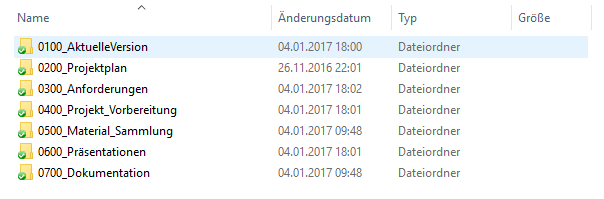
\includegraphics[scale=1]{projectdefinition/Bilder/FolderStructure}
\caption{Ordner Struktur Projekt}
\label{fig:folderStruct}
\end{figure}
Für Dokumente, welche gemeinsam bearbeitet wurden, erstellte man Vorlagen. Diese konnten separat erstellt werden und wurden anschließend zusammengeführt. Dies ermöglichte einen einheitlichen Stil der Dokumente.
